\section{Implementation}

The simulator is implementated in Golang, also known as just Go. 
Go is an opensource programming language supported by google, that boasts an impressive performance.
Choosing Go instead of any other programming language was very much just a roll of the dice.
Even if Go is choosen from chance, it does however, help implement the design quite well. 

\subsection{Structure}
Go operates with packages that by convention is structured by folders. 
To facilitate an extensible and maintainable simulator, the simulator is build as a RS32I package.
The simulator package is then used in a main package that handles loading binary and displaying outputs et cetera.

\dirtree{%
.1 src.
.2 main.go.
.2 simulator (RS32I). 
.3 arithmetic.go.
.3 arithmetic\_test.go.
.3 binary.go.
.3 (etc..).
}

With this structure, new extensions could be implemented and used in the main package.

\subsection{Simplicity}

Registers and memory is implemented by plain global arrays.
The program counter is also a global variable.
To simplify the implementation, registers are using uint32 to make using Go's standard "encoding/binary" library easier.

\begin{figure}[h]
\begin{minted}[linenos]{golang}
var (
    Pc  int32
    Reg []uint32
    Mem []byte
)
\end{minted}
\end{figure}

Running a simulation of a binary file is then simply implemented by loading binary file into Mem array, then execute instructions in a while loop.
\begin{figure}[h]
\begin{minted}[linenos]{golang}
for s.Pc < programLength && !s.ECALL {
    instrBs := s.Mem[s.Pc : s.Pc+4] // Fetch instructions from memory
    inst := s.Decode(instrBs)       // Decode instruction from binary
    inst.Execute()                  // Execute operation from instruction
    s.Pc += 4                       // Increment program counter
}
\end{minted}
\end{figure}

\newpage

\begin{wrapfigure}[14]{r}{0.4\textwidth}
    \centering
    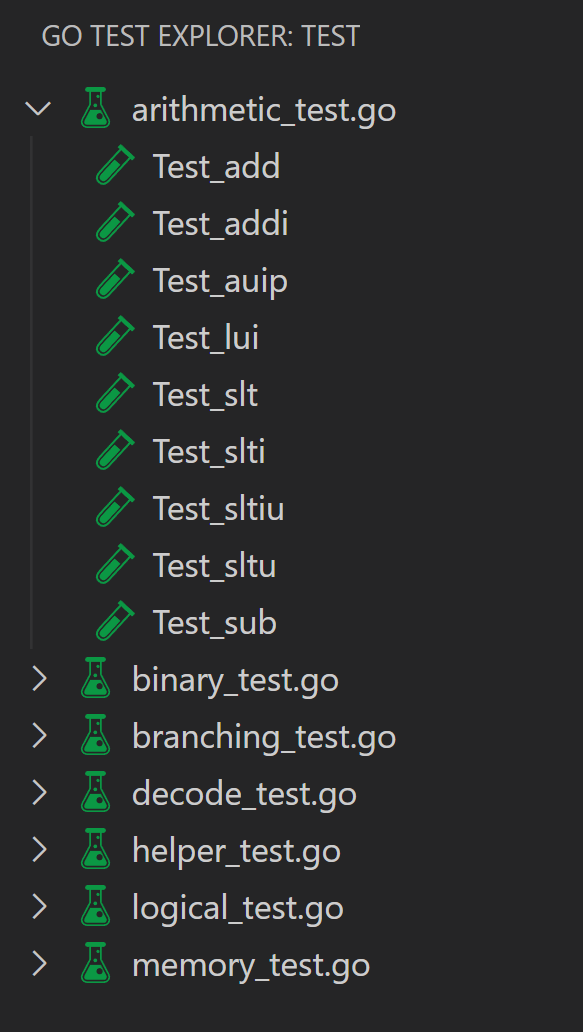
\includegraphics[width=0.4\textwidth]{images/test.png}
\end{wrapfigure}

\subsection{Testing}

Golang provides a testing framework as part of the standard language toolchain.
By convention, tests are automatically picked up for files postfixed with "\_test".
The test as described in the Testability design section \ref{test} can be created as follows.

Given the $Add$ function exists in \textbf{arithmetic.go}, then a test file is created named: \textbf{arithmetic\_test.go}.
The following test code is then put in the test file:
\begin{figure}[h]
\begin{minted}[linenos]{golang}
func Test_add(t *testing.T) {
    Reg[11] = 5
    Reg[12] = 3
    add(10, 11, 12)
    assert(Reg[10], 8, t)
}
\end{minted}
\end{figure}

Using command line, the tests can be executed by the following command (given source root as working directory):

\begin{figure}[H]
\begin{minted}[linenos]{bash}
$ go test ./simulator/
ok      ./simulator 0.246s
\end{minted}
\end{figure}

Besides the command line, there is various integrations that exists. Like the visual studio code extension view shown in the screenshot to the right.


\newpage